\chapter{Introduction}
\label{cha:chapter1}
\section{Motivation}
In recent years, machine learning  has been increasingly involved in almost every aspect of our life, for example recommendation systems on e-commerce sites, cancer diagnosis, or self-driving car. This developments can not be achieved without intelligent algorithms behind. Due to great amount of data and more efficient computational resources, a certain type of machine learning, called neural networks, are directly benefitted and are able to achieve much better performance that traditional machine learning techniques. As a result, many intelligent systems that we use today somehow rely on them.


In short, neural networks are algorithms that are inspired by human. They have units, called neurons, arranged in layers working together to transform input to a desired output. When networks contains many layers, they are referred as deep learning. Connections between neurons define this transformation and will be learned from data. Because the transformation is typically in high dimensional space and built specifically to a certain problem, it is not obvious to us how trained neural networks utilize an input and make a prediction.  This lack of understanding  raises concerns and questions to the machine learning community and consumers. One major concern is trust to neural network systems, in particular, how we can ensure that the systems will work as we expect. Secondly, without knowing how neural networks process input to the output results in great amount of trials and errors to configure the systems to achieve expected performance.

Several methods have been proposed by researchers in order to better understand or explain how neural networks transforms input to output. Although these work has demonstrated promising results on neural networks, more specifically feed-forward architectures, there is still only a few applications of these methods to recurrent architecture. These recurrent neural networks are considerably important and have been powering almost machine learning systems processing sequential data, such as machine translation and natural language understanding. Therefore, applications of these explanation techniques to recurrent neural networks need to be explored. This results will also enable us to propose adjustments to recurrent architectures such that they are more explainable.


\section{Objective \& Scope}
The goal of this thesis is to  study how structure of recurrent neural networks affect the quality of explanations produced by various explanation techniques. In particular, the technique that will be experimented are sensitivity analysis(SA), guided backprop(GB), Layer-Wise Relevance Propagation(LRP) and deep Taylor decomposition(DTD). Our study is based on an artificial classification problem. This problem is specifically constructed such that  knowledge of ground truth explanations is available and we can perform qualitative and quantitative measurement accordingly.

The main hypothesis of this thesis is that recurrent neural networks with more layers are more expressible than fewer layers. We extensively conduct experiments on various configurations of recurrent neural network architectures to verify the result. We also propose a adjustment to one of the state-of-the-art recurrent neural network architectures such that it can be explained by the techniques mentioned above.

Lastly, as the primary goal is to study explainability of recurrent neural networks, we do not seek to train models to achieve the state-of-the-art performance. We rather train them to reach a certain level of performance. We assume that models operating in this level would  produce comparable explanations.


%assumption relu? ... 
%
%not care performance much ..
%
%our hypothesis ... 
%
%artificial problems ... 


\section{Dataset}


\subsection{MNIST}
MNIST\cite{LeCunMNISThandwrittendigit2010} is one of the most popular dataset that machine learning partitioners use to benchmark machine learning algorithms. The dataset consists of 60,000 training and 10,000 testing samples. Each sample is a grayscale 28x28 image of a digit between from 0 to 9. 

\begin{figure}[!hbt]
\centering
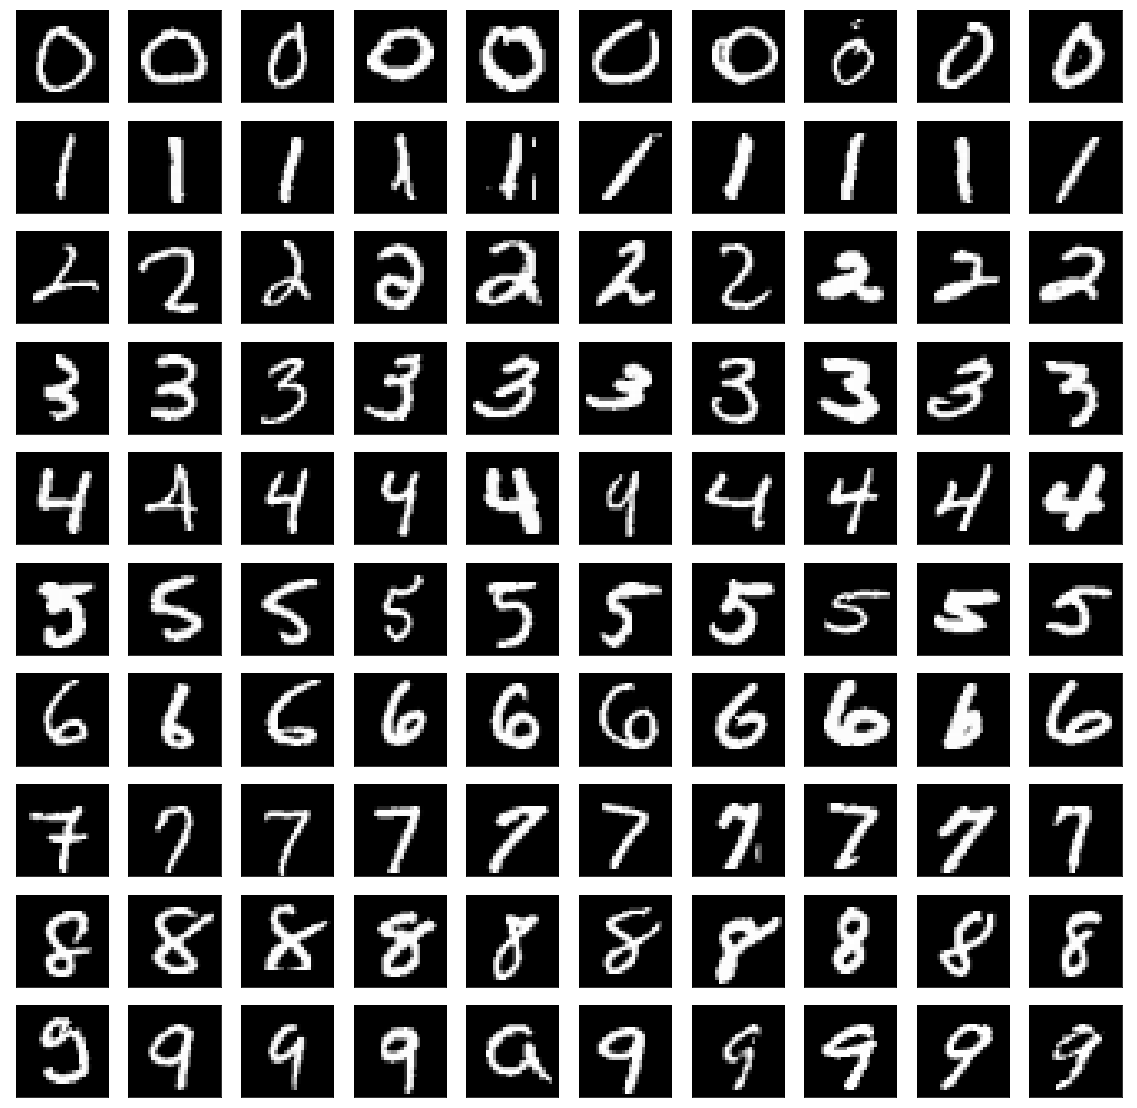
\includegraphics[width=0.6\textwidth]{mnist}
\caption{Samples in MNIST}
\label{fig:mnist_samples}
\end{figure}

State-of-the-art algorithms can classify MNIST with accuracy higher than 0.99, while classical ones, such as SVC or RandomForest, are able to achieve around 0.97\cite{XiaoFashionMNISTNovelImage2017}.


\subsection{FashionMNIST}

Xiao et. al.\cite{XiaoFashionMNISTNovelImage2017} propose a novel dataset, called FashionMNIST dataset, as a replacement of MNIST dataset for benchmarking machine learning algorithms.  According to \cite{XiaoFashionMNISTNovelImage2017},  Fashion-MNIST brings more challenging to the problem and more representative to modern computer vision tasks. It contains images of fashion products from 10 categories. Fashion-MNIST is comparable to MNIST in every aspects, such as the size of training and testing set, image dimension and data format, hence one can easily  apply existing algorithms that work with MNIST to Fashion-MNIST without any change.

\begin{figure}[!hbt]
\centering
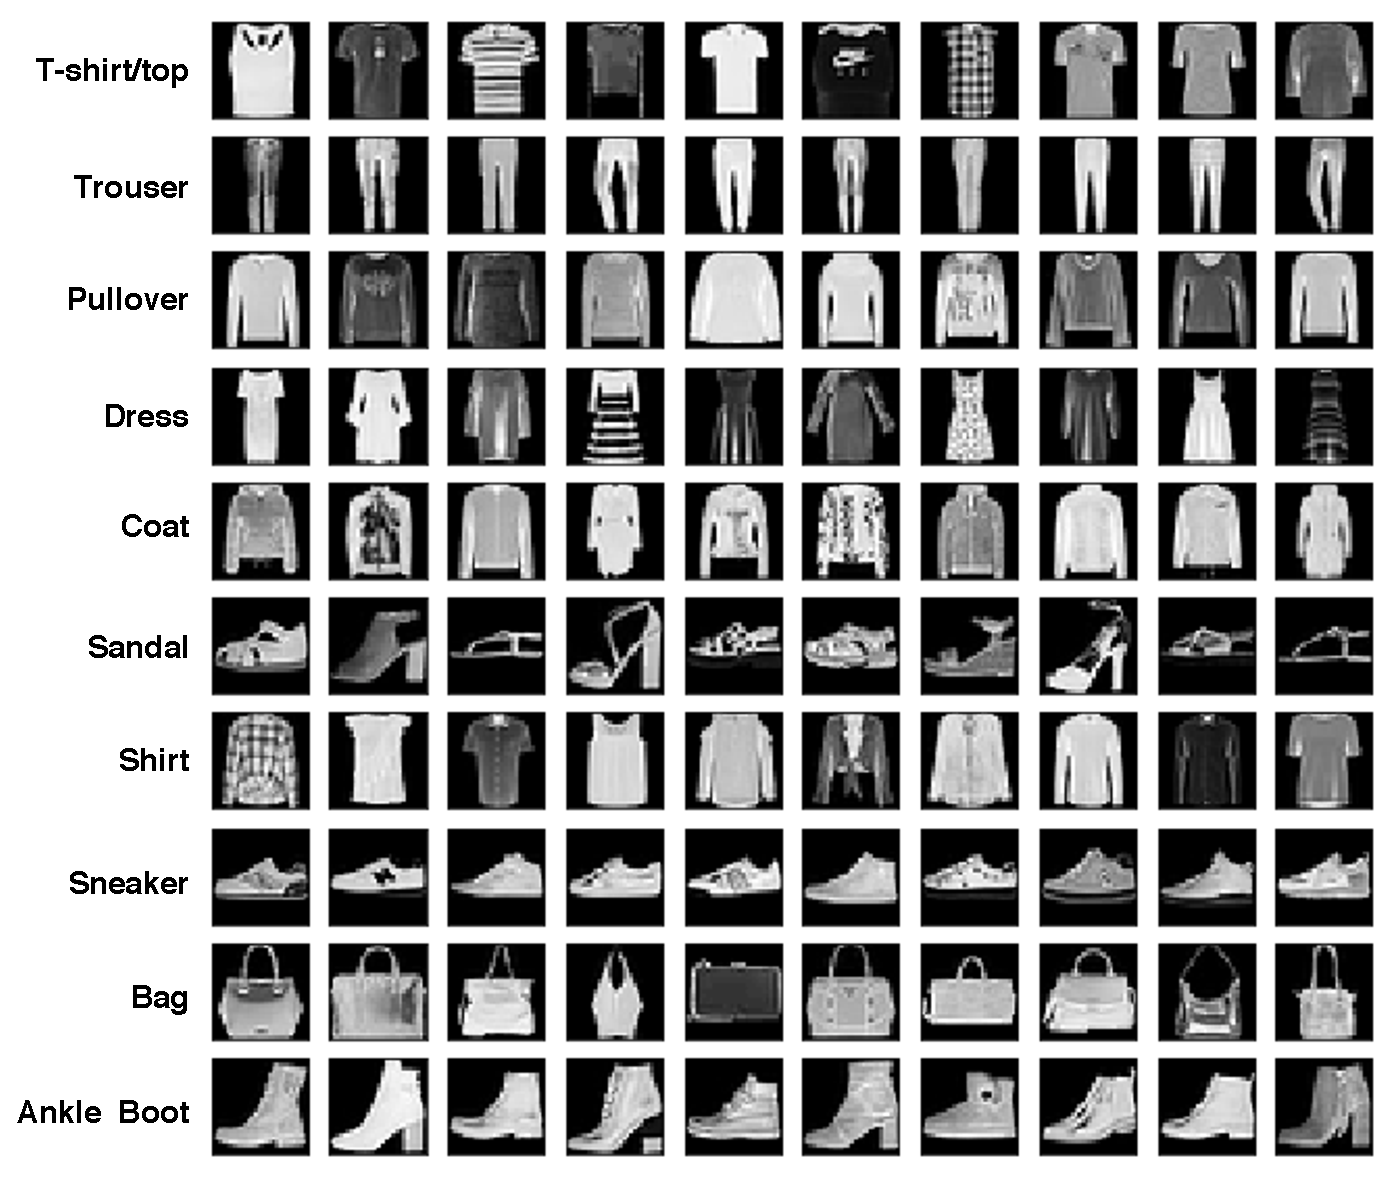
\includegraphics[width=0.65\textwidth]{sketch/fmnist_samples}
\caption{Samples in FashionMNIST}
\label{fig:fashion_mnist_samples}
\end{figure}

\cite{XiaoFashionMNISTNovelImage2017} also reports benchmarking results of classical machine learning algorithms on Fashion-MNIST. On average, they achieve accuracy between 0.85 to 0.89. According to Fashion-MNIST's page\footnote{https://github.com/zalandoresearch/fashion-mnist}, A. Brock reports the state-of-the-art result  with 0.97 accuracy using Wide Residual Network(WRN)\cite{ZagoruykoWideResidualNetworks2016} and standard data preprocessing and augmentation.


\section{Outline}
The thesis is organized as follows :
\begin{itemize}
	\item \textbf{Chapter \ref{cha:chapter2}} provides a brief literature survey and related work in the direction towards explaining neural networks.
	\item \textbf{Chapter \ref{cha:chapter3}} summaries necessary backgrounds in neural networks and explanation techniques that are discussed in the thesis.
	\item \textbf{Chapter \ref{cha:chapter4}} is devoted to experimental results.
	\item \textbf{Chapter \ref{cha:chapter5}} concludes the results and discusses challenges as well as future work.
\end{itemize}

%
%This chapter should have about 4-8 pages and at least one image, describing your topic and your concept. Usually the introduction chapter is separated into subsections like 'motivation', 'objective', 'scope' and 'outline'.
%
%\section{Motivation\label{sec:moti}}
%
%Start describing the situation as it is today or as it has been during the last years. 'Over the last few years there has been a tendency... In recent years...'. The introduction should make people aware of the problem that you are trying to solve with your concept, respectively implementation. Don't start with 'In my thesis I will implement X'.
%
%\section{Objective\label{sec:objective}}
%
%What kind of problem do you adress? Which issues do you try to solve? What solution do you propose? What is your goal?
%'This thesis describes an approach to combining X and Y... The aim of this work is to...'
%
%\section{Scope\label{sec:scope}}
%
%Here you should describe what you will do and also what you will not do. Explain a little more specific than in the objective section. 'I will implement X on the platforms Y and Z based on technology A and B.'
%
%Conclude this subsection with an image describing 'the big picture'. How does your solution fit into a larger environment? You may also add another image with the overall structure of your component.
%
%'Figure \ref{fig:intro} shows Component X as part of ...' 
%\\
%\begin{figure}[htb]
%  \centering
%  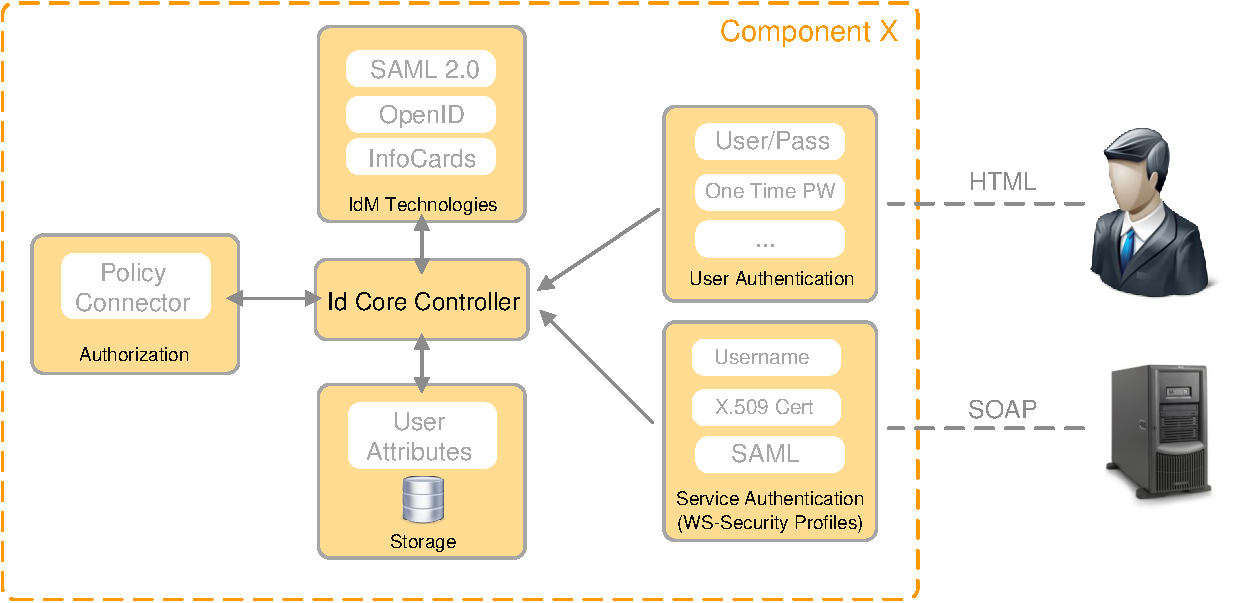
\includegraphics[width=9cm]{intro_example.pdf}\\
%  \caption{Component X}\label{fig:intro}
%\end{figure}
%
%\section{Outline\label{sec:outline}}
%
%The 'structure' or 'outline' section gives a brief introduction into the main chapters of your work. Write 2-5 lines about each chapter. Usually diploma thesis are separated into 6-8 main chapters. 
%\\
%\\
%\noindent This example thesis is separated into 7 chapters.
%\\
%\\
%\textbf{Chapter \ref{cha:chapter2}}  Neural Network and Explainability foudation
%%is usually termed 'Related Work', 'State of the Art' or 'Fundamentals'. Here you will describe relevant technologies and standards related to your topic. What did other scientists propose regarding your topic? This chapter makes about 20-30 percent of the complete thesis.
%\\
%\\
%\textbf{Chapter \ref{cha:chapter3}} Architecture
%%analyzes the requirements for your component. This chapter will have 5-10 pages.
%\\
%\\
%\textbf{Chapter \ref{cha:chapter4}} Experiments
%%Ais usually termed 'Concept', 'Design' or 'Model'. Here you describe your approach, give a high-level description to the architectural structure and to the single components that your solution consists of. Use structured images and UML diagrams for explanation. This chapter will have a volume of 20-30 percent of your thesis.
%\\
%\\
%\textbf{Chapter \ref{cha:chapter5}} Conclusion and future work
%%describes the implementation part of your work. Don't explain every code detail but emphasize important aspects of your implementation. This chapter will have a volume of 15-20 percent of your thesis.
%%\\
%\\
%%\textbf{Chapter \ref{cha:chapter6}} is usually termed 'Evaluation' or 'Validation'. How did you test it? In which environment? How does it scale? Measurements, tests, screenshots. This chapter will have a volume of 10-15 percent of your thesis.
%%\\
%%\\
%%\textbf{Chapter \ref{cha:chapter7}} summarizes the thesis, describes the problems that occurred and gives an outlook about future work. Should have about 4-6 pages.